\documentclass[../main.tex]{subfiles}

\begin{document}

The main "theme" of this PhD is understanding the best approach to embedding information before input into a transformer-based active learning system.  This is based on the research gaps identified, such as short context windows given with previous transformer-based TAR research and its strict adherence to faithful replication of how humans screen documents for inclusion into SRs.  

Research questions identified through this literature review can be summarised into:
\begin{itemize}
    \item Does utilising a larger context window, or domain-pretrained models improve BERT performance in the CAL process?
    \item Does the provision of additional metadata, such as a citation network, improve model performance in CAL?
    \item Does utilising decoders as embedders rather than encoders result in better CAL performance?
\end{itemize}

\subsection{Enabling fair comparison}

So far, the existing literature represents documents as a concatenation of the title and abstract, which is then embedded using models such as 'bert-based-uncased'. A significant limitation is a fixed input of 512 tokens. If we concatenate the title and abstract of the CLEF dataset, this leads to a truncation of the input, as demonstrated in Table \ref{tab:clef_token_limits}\footnote{https://github.com/afletcher53/bert-clef-diff}.  If we further consider how abstracts are formatted, with it approximating the logical structure of the content (background, method, results, conclusions), then the likely truncation of the conclusion, which outlines the vital contribution of that paper on the topic, would undoubtedly lead to poorer performance. Compare this to the TF-IDF approaches of Auto TAR, which will still likely contain important missing words from those documents, making the comparison ultimately unfair. 

\begin{table}
    \centering
    \begin{tabular}{|c|c|}
        \hline
        Statistic & Value  \\ \hline
         Average Percentage of Lost words & 21.18\%  \\ \hline
         Average number of words lost &  66.94 \\ \hline
        Maximum percentage of lost words &  87.50\% \\\hline
    \end{tabular}
    \caption{Statistics demonstrating limitation of the 512 embedding process on the CLEF dataset, code generated by Author.}\footnote{https://github.com/afletcher53/bert-clef-diff} 
    \label{tab:clef_token_limits}
\end{table}

The author will make use of existing approaches that have been developed to deal with a long context, such as LongFormer or Big Bird, which are available with an expanded token input length (up to 4096 tokens).

Longformer is a model that adapts RoBERTa to accept longer token inputs \cite{beltagy_longformer_2020}. This was achieved through the introduction of an attention mechanism that grows linearly with the length of the sequence through a sliding window of size w, changing the computational complexity of query generation, the key values from \(O(n^2)\) (in original transformer implementation) to \(O(nw)\), where n is the length of the sequence and w is the average window size. This resulted in a minor increase in accuracy compared to the original RoBERTAa base. Models have been made available for use, which include a 4096 token window, which can be fine-tuned on datasets (such as all the data returned from the previous screening stage) and optimised for smaller token windows\footnote{https://colab.research.google.com/drive/$1m22nj5A3g-KigoHT1xPgxe_0uYX8HPfA?$usp=sharing}. There are more domain-specific versions of long former available, such as clinical long former \cite{li_comparative_2023}, which have been further trained in MIMIC 3 clinical notes \footnote{https://huggingface.co/yikuan8/Clinical-Longformer}.

\begin{figure}
    \centering
    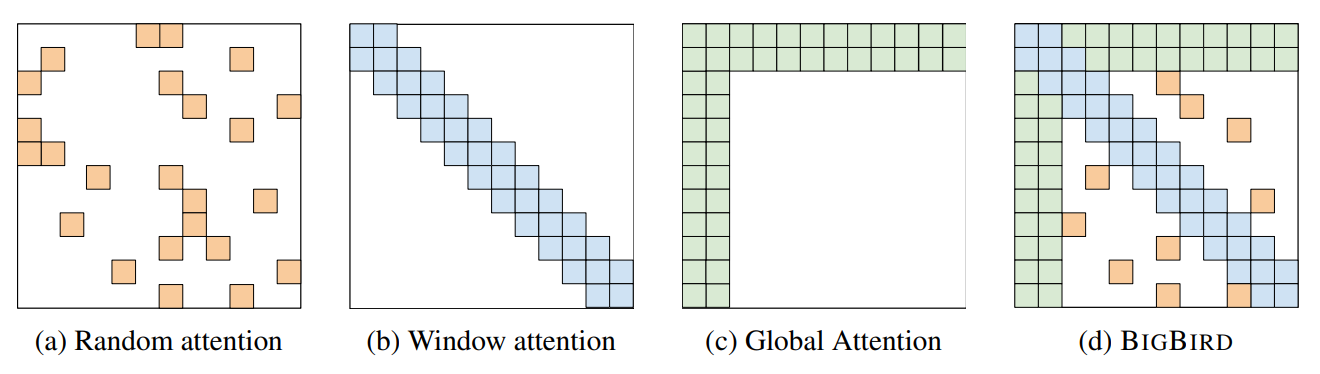
\includegraphics[width=1\linewidth]{sections//images/Differing Attention Mechanisms.png}
    \caption{Differing attention mechanisms: Longformer utilises window attention, while Big Bird utilises all 3. Note that the original attention mechanism utilises all squares (including white ones)}
    \label{fig:attention_mechanism}
\end{figure}

Alternatives include the more recently introduced Big Bird \cite{zaheer_big_2021}, which attempts to combine global attention, window attention, and random attention - see Figure \ref{fig:attention_mechanism}, and resulted in an improvement of the then state of the art by 5\% in document classification. 

Additionally, BERT models run so far have used a non-domain-specific pre-trained model, despite them existing (such as BioBERT).

This RQ is deliberately limited in scope. The design of subsequent RQs depends on advances made within RQ1 (as if a longer contextual representation improves the TAR process, it is deemed likely to result in improvements within the other approaches). Additionally, the technical ability gained from undertaking this RQ, such as the utilisation of BERT and replication of experimental approaches, provides a solid basis for further RQs, which will attempt to augment these processes further.

\textbf{Research needed:} To address this research gap, the author proposes replicating previous experiments, including the "Goldilocks reproduce" study, and comparing them with models utilizing larger context windows. This comparison aims to determine whether these extended context approaches yield significant improvements. The research will fine-tune each long-context model using either a) the complete set of document candidates for individual SRs within the datasets or b) the entire corpus of document candidates across all SRs in the datasets. The choice between these approaches will depend on time and computational constraints. This methodology will enable a comprehensive evaluation of the potential benefits of larger context models in SR automation, and hopefully demonstrate a fairer comparison.

\subsection{Limited feature useage}

The medical TAR AL process aims to emulate human decision-making in SRs. Traditionally, these approaches have mirrored the human workflow: screening titles and abstracts are first, followed by full-text analysis. This sequential method minimises the time-consuming and resource-intensive full-text review phase of human reviewers.

However, computational approaches are not subject to the same constraints as human reviewers. By limiting machine learning algorithms to title and abstract screening, we may inadvertently restrict their potential to perform this task effectively.
Consider, for example, the value of analysing author-related information. As demonstrated by the author's previous research, metadata, such as an author's name, can determine if research is valuable. Some authors consistently produce high-quality research within specific domains, making their publications more likely to meet the inclusion criteria for SRs.
To further this point, each article will have a list of references. These references create a citation network where you can trace significant research back to its source, which can be used to judge its significance.
By confining AL algorithms to title and abstract data, we exclude potentially crucial information that could inform screening decisions. It is important to note that the intention is not to eliminate the human full-text screening phase of the SR process. Instead, the goal is to use all available information during the initial screening phase to identify papers that warrant full-text review more accurately.
This approach could improve the efficiency and precision of the overall SR process, allowing computational methods to use a broader range of data points to make preliminary screening decisions. The TAR process is meant to emulate humans, yet ultimately its goal is to surpass them. 

Many tools are available to explore the metadata for medical papers, such as Open Alex \cite{priem_openalex_2022}, which provides granular access to all available metadata, such as citations, references, author metadata, etc. 

Different approaches exist to augment information for inclusion within language models such as BERT. BERT was used to process text features from book blurbs and titles, which were then concatenated with metadata features (such as number of authors, academic titles, word counts, and more)\cite{ostendorff_enriching_2019}. Crucially, the authors also included pre-trained graph embeddings derived from the Wikidata knowledge graph, representing authors and their relationships. This combined representation (text features, metadata, and graph embeddings) was used for classification tasks.

The results demonstrated that the incorporation of metadata features and author embeddings led to better performance for both classification tasks compared to a text-only approach. For a coarse-grained classification task with eight labels, the enriched BERT model achieved an F1-score of 87.20. For a more detailed classification task with 343 labels, the model achieved an F1-score of 64.70. These results outperformed other configurations, including a baseline model using Logistic Regression and TF-IDF vectors.

Additionally, the concept of TwinBERT, which employs two parallel BERT models to separately process text and metadata, has been explored to address the token limit constraints of BERT. This approach showed promising results, particularly in improving recall and precision using textual and contextual information effectively \cite{wolff_enriched_2024}. This RQ is very closely tied to the first one (and could correctly been seen as enabling a fair comparison); however, because it augments the existing title and abstract screening phase, and can potentially build upon any advances found in RQ1, it has been separated.

\textbf{Research needed:} To address this research gap, the author proposes a series of experiments that append metadata from Openalex to the existing data (title/abstract) and then use either TwinBERT, or concatenation of the BERT representation approaches within Active learning. The exact architecture for this is currently undetermined.

\subsection{Decoders as text encoder}

To date, all approaches utilising LLMs within the TAR process employ encoder architectures, such as BERT, to represent documents. This is logical because encoder architectures are trained in masked language modelling (MLM) and, in some cases, next-sentence prediction, which facilitates effective document representation. In contrast, decoder architectures are trained on next token prediction, enabling them to learn from both preceding and following tokens, thus leveraging information from the entire context rather than a masked subset. Recent studies, such as LLM2Vec\cite{behnamghader_llm2vec_2024}, have demonstrated that decoder-derived embeddings outperform those from encoder-only models across various tasks, including classification. However, no research in active learning has yet explored the potential of decoder-derived embeddings.

\textbf{Research Needed: }To address this gap, the author proposes selecting a pre-trained decoder-only LLM, such as LLaMA-2-7B, applying the LLM2Vec transformation to it, and using the transformed model to represent documents. Subsequently, the traditional active learning loop can be performed using classifiers such as logistic regression.

\subsection{Stretch RQs}

As discussed in the subsequent timeline section, time has been allocated to pursue further developments that might arise while undertaking this Ph.D. The stretch RQs have yet to be fully formulated; however, currently the author is exploring:

\textbf{Using Mixtures of Experts (MOE) in SR TAR process} \cite{cai_came_2023}. MOE attempts to use multiple models, each of which specialises in a specific portion of the data (which in information recall we could consider models optimised for true precision, true recall, etc.) and then using a router to decide which expert should handle each input data. Both experts and router are trained simultaneously. This idea could be further developed into a policy selection MOE, which would allow policy selection that adapts to the already known data pool.

\textbf{Using Query by Committee (QBC)} in SR TAR process\cite{hino_active_2022}. In this approach, a committee of models is used to answer the question on if a document should be marked as included within SR, with a measure, such as vote entropy or kullback-eibler divergence, used to determine the aggregated committee result. QBC is different from MOE, as it does not necessarily use specialised models or a router, rather, an ensemble of diverse models to make decisions, with the more disagreed about input being sent to humans for classification.

\textbf{Elimination/minimisation of oracle} within the SR TAR process. In the TAR  process for SR, we employ sampling policies (\(\pi\)) to select documents for human relevance judgement. These policies, such as uncertainty sampling, aim to present the most challenging examples for the LR model to classify. We currently use the sigmoid output of the LR model as a proxy for classification certainty, with the 0.5 mark on the sigmoid curve representing maximal uncertainty for the LR model. However, this approach has limitations. The sigmoid output more accurately reflects the LR model's uncertainty, not the true difficulty for human classification. As a result, we may inadvertently present "easy-to-classify" documents to the human oracle, leading to inefficient use of human expertise. The author proposes incorporating more sophisticated models into the document selection process. This improvement involves introducing a pre-screening phase using advanced language models (e.g., GPT-4, Gemini, Claude). These models would analyse candidate documents before human review. Measures such as Shannon entropy of the model responses can be used to gauge true classification difficulty, only presenting documents to the human oracle when deemed necessary based on this analysis.

This approach offers several advantages. It balances computational resources with human expertise, potentially reduces the number of "easy" documents sent for human review, and reserves human judgment for truly ambiguous or complex cases. By implementing this enhanced process, the author aims to optimise the efficiency and effectiveness of the SR TAR workflow, making better use of both computational and human resources.

\end{document}
